\chapter{Minimum-basis H$_2$} \label{app:mbh2}
To derive the Hartree-Fock equations, we use a Slater determinant to evaluate the total energy, then minimize it. Consider $N$ spinless fermions, labeled using $i,j,k,\dots$, in $N$ orbitals $\chi_a,\chi_b,\dots,\chi_N$. Given determinant wavefunction $\ket{\Psi_0}=\ket{\chi_a\chi_b\dots\chi_N}$ and electronic Hamiltonian made up of only one- and two-electron terms $\mathcal{H}=\sum\limits_{i=1}^N h(i) + \sum\limits_{i=1}^N\sum\limits_{j>i}^N v(i,j)$. The total energy is
\begin{align} \label{eq:sdet-energy}
E= \sum\limits_{a=1}^N [a|h|a] + \frac{1}{2}\sum\limits_{a,b=1}^N [aa|bb] - [ab|ba],
\end{align}
where $[a|h|a]$ denotes, and $[aa|bb]$ denotes~\cite{Szabo1996}.

Constraint minimization of eq.~(\ref{eq:sdet-energy}) with the extra requirement that each spin orbital is doubly occupied leads to the restricted Hartree-Fock (RHF) Fock operator. Its first $N/2$ eigenvectors are the spin orbitals in the lowest-energy Slater determinant. The lowest energy value can be obtained by a weighted sum of its eigenvalues according to the occupation of the spin orbitals.

Instead of starting with the tedious derivation of the Fock operator and its iterative numerical solver, I will first show a concrete application of RHF to minimum-basis hydrogen molecule (H$_2$). %The minimum basis consists of two 1s functions, one centered at each nucleus $\{\phi_\mu\}$, $\mu=1,\dots,K$, where $K=2$.
On p. 140 of A. Szabo and N. S. Ostlund, the restricted Fock operator in any basis $\{\phi_\mu\}$ is written as
\begin{align}
F_{\mu\nu} = \hcore + \sum\limits_{a=1}^{N/2} 2(\mu\nu|aa) - (\mu a|a\nu),
\end{align} % (3.148)
where $a$ labels molecular orbitals, which are eigenstates of the Fock operator. We immediately note that the Fock operator is a peculiar one-electron operator that depends on its own eigenstates. A self-consistent solution to $F_{\mu\nu}$ typically involves guessing, checking and iterating.

$\hcore$ is the one-electron part of the Hamiltonian expressed in the given basis % (3.149)
\begin{align} \label{eq:hf-hcore}
\hcore = \int d\bs{r}_1 \phi_\mu^*(\bs{r}_1)\left(
-\frac{1}{2}\nabla_1^2-\sum\limits_A \dfrac{Z_A}{\vert\bs{r}_1-\bs{R}_A\vert}
\right)  \phi_\nu(\bs{r}_1).
\end{align}
The two-electron integral notation $(\mu\nu|\lambda\sigma)$ is defined by eq.~(3.155) in Szabo
\begin{align} \label{eq:hf-eri}
(\mu\nu|\lambda\sigma) = \iint d\bs{r}_1 d\bs{r}_2 \phi_\mu^*(\bs{r}_1)\phi_{\nu}(\bs{r}_1)
\frac{1}{\vert\bs{r}_1-\bs{r}_2\vert}
\phi_\lambda^*(\bs{r}_2)\phi_\sigma(\bs{r}_2).
\end{align}
The first term in the sum of eq.~(\ref{eq:roothaan-fock})
\begin{align}
J_{\mu\nu} \equiv (\mu\nu|aa)
\end{align}
is often called the Coulomb or direct operator, because it describes the Classical density-density interaction of charged particles having density distribution $\phi_a^*(\bs{r}_2)\phi_a(\bs{r}_2)$. The second term
\begin{align}
K_{\mu\nu} \equiv (\mu a|\nu a)
\end{align}
is the exchange operator and has no classical interaction. The exchange-correlation contribution to the Fock matrix is sometimes called the Hartree-Fock effective potential operator
\begin{align}
\ksveff\equiv 2J_{\mu\nu} - K_{\mu\nu}.
\end{align}

Suppose each molecular orbital $a$ is written as a linear combination of the basis functions
\begin{align}
\psi_a = \sum\limits_{\mu=1}^K C_{\mu a} \phi_\mu,
\end{align}
then the Fock operator can be written as (from Roothaan equations)
\begin{align} \label{eq:roothaan-fock}
F_{\mu\nu} = \hcore + \sum\limits_{\lambda\sigma} P_{\lambda\sigma} \left[
(\mu\nu|\sigma\lambda) - \frac{1}{2}(\mu\lambda|\sigma\nu)
\right],
\end{align} % (3.154)
where $P_{\lambda\sigma}=2\sum_{a=1}^{N/2} C_{\lambda a}C_{\sigma a}^*$ is the density matrix. % (3.145)

Conceptually, the simplest approach would be to use the ground-state wavefunctions of the two hydrogen atoms as the basis for the hydrogen molecule. We can guess the ground-state wavefunction of the hydrogen molecule. First, the spins of the two electrons anti-align, so they are distinguishable particles. Second, due to symmetries imposed by the two protons, the ground state must be equal superposition of the two basis functions. Third, the lowest-energy solution has no node. Therefore, the ground state of H$_2$ in the minimum basis is
\begin{align}
\psi_1 = \left[2(1+S_{12})\right]^{-1/2} \left(
\phi_1 + \phi_2
\right),
\end{align}
where $S_{12}=\braket{\phi_1|\phi_2}$. That is $C_{11}=C_{21}=\left[2(1+S_{12})\right]^{-1/2}$
\begin{align} \label{eq:h2-pmat}
P_{\lambda\sigma} = \left[2(1+S_{12})\right]^{-1/2}\left(\begin{array}{cc}
1 & 1 \\
1 & 1
\end{array}\right).
\end{align}
This guess was obtained as early as 1927 by V. W. Heitler and F. London~\cite{Heitler1927}. Unfortunately, the multi-center integrals eq.~(\ref{eq:hf-hcore}) and (\ref{eq:hf-eri}), needed to evaluate the total energy, have no analyical form in the basis of Slater type orbitals (STOs) (see thesis of Michał Lesiuk). Thus, Heitler-London used an upper bound to approximate the two-electron integral and obtain a bond length of 1.5 bohr and binding energy of 2.5 eV, noticeably different from the experimental values of 1.4 bohr and 4.5 eV.

In modern quantum chemistry, instead of directly approximating the integrals, we analytically evaluate the integrals by approximating each basis function as a sum of Gaussians. This reduces the multi-center integrals to single-center integrals, because a product of Gaussians centered on different atoms is also Gaussian but with a different center. The so-called STO-3g basis expresses a STO as a sum of 3 ``primitive Gaussians'' (see eq. (3.225) of Szabo). Using this basis, the bond length and binding energy become 1.35 bohr and 3.2 eV, having roughly half the discrepancy with experiment when compared to the Heitler-London values.

%\begin{align}
%\chi_{nlm}(r, \theta, \phi;\zeta) \equiv \dfrac{(2\zeta)^{n+1/2}}{\sqrt{(2n)!}}
%r^{n-1}e^{-\zeta r} Y_{lm}(\theta, \phi).
%\end{align}
%\begin{align}
%g(r; \sigma) = \dfrac{1}{\sigma\sqrt{2\pi}} e^{-\dfrac{r^2}{2\sigma^2}}.
%\end{align}

Figure~\ref{fig:sto-3g} shows the STO-3g basis compared to the exact STO it approximates
\begin{align}
\chi(r)\equiv \left(\dfrac{\zeta^3}{\pi}\right)^{1/2} e^{-\zeta r} \approx \phi(\bs{r}) = \sum\limits_{i=1}^3 c_i \left(\dfrac{2\alpha_i}{\pi}\right)^{3/4} e^{-\alpha_ir^2},
\end{align}
where the exponents $\bs{\alpha}$ and coefficients $\bs{c}$ are given below:
\begin{figure}[h]
\begin{minipage}{0.29\textwidth}
\begin{tabular}{cc}
\toprule
$\alpha$ & $c$ \\
\midrule
3.42525091 & 0.15432897 \\
0.62391373 & 0.53532814 \\
0.16885540 & 0.44463454 \\
\bottomrule
\end{tabular}
\end{minipage}
\begin{minipage}{0.59\textwidth}
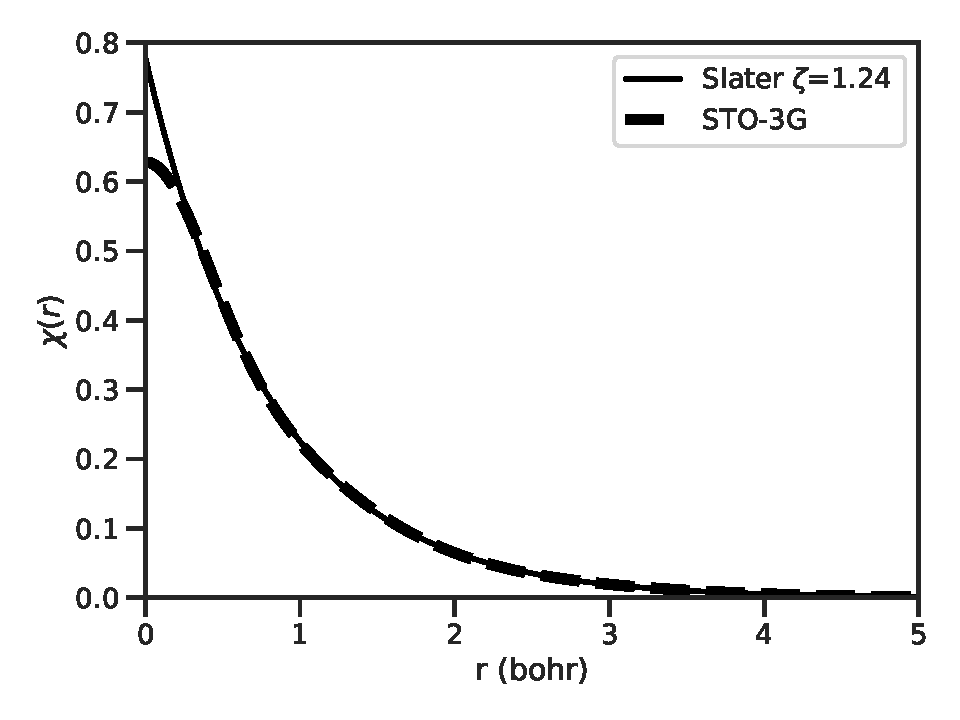
\includegraphics[width=\textwidth]{sto-3g}
\end{minipage}
\caption{STO-3G}
\label{fig:sto-3g}
\end{figure}

For H$_2$, the STO-3G basis consists of only two 1s functions, each centered around a nucleus.
\begin{align}
\left\{\begin{array}{l}
\phi_1(\bs{r}) = \sum\limits_{i=1}^3 c_i \left(\dfrac{2\alpha_i}{\pi}\right)^{3/4} e^{-\alpha_i\vert\bs{r}-\bs{R}_1\vert^2} \\
\phi_2(\bs{r}) = \sum\limits_{i=1}^3 c_i \left(\dfrac{2\alpha_i}{\pi}\right)^{3/4} e^{-\alpha_i\vert\bs{r}-\bs{R}_2\vert^2}
\end{array}\right.,
\end{align}
where $\bs{R}_1=\bs{0}$, and $\bs{R}_2=1.4~\bs{\hat{z}}$ bohr near equilibrium. At 1.4 bohr separation, the kinetic and the electron-ion interaction matrices evaluate to
\begin{align}
T_{\mu\nu}\equiv\braket{\phi_\mu|-\frac{1}{2}\nabla^2|\phi_\nu} =
\left(\begin{array}{cc}
0.76003188 & 0.23645465 \\
0.23645465 & 0.76003188
\end{array}\right), \\
V_{\mu\nu}\equiv\braket{\phi_\mu|\sum\limits_{i=1}^{2}\dfrac{1}{\vert\bs{r}-\bs{R}_i\vert}|\phi_\nu} = \left(\begin{array}{cc}
-1.88044088 & -1.19483461 \\
-1.19483461 & -1.88044088
\end{array}\right),
\end{align}
which sum to the 1-electron hamiltonian $\hcore$ by eq.~(\ref{eq:hf-hcore})

Eigenvectors of $\hcore$ are typically used to construct the initial density matrix to start a self-consist solution of the Hartree-Fock equations. However, in the case of H$_2$, these eigenvectors coincide with the final solution, so we obtain the converged density matrix with no iteration from eq.~(\ref{eq:h2-pmat})
\begin{align}
C_{\mu 1} = \left(\begin{array}{c}
0.70710678 \\ -0.70710678
\end{array}\right);
~P_{\mu\nu} = \left(\begin{array}{cc}
0.60265716 & 0.60265716 \\
0.60265716 & 0.60265716
\end{array}\right).
\end{align}
Finally, we can evaluate the so-called electron repulsion integrals (eris) and the Fock matrix eq.~(\ref{eq:roothaan-fock})
\begin{table}[h]
\centering
\begin{tabular}{ccccc}
\toprule
$\mu$ & $\nu$ & $\lambda$ & $\sigma$ & $(\mu\nu|\lambda\sigma)$\\
\midrule
1 & 1 & 1 & 1 & 0.774605930 \\
1 & 1 & 1 & 2 & 0.444107650 \\
1 & 1 & 2 & 2 & 0.569675915 \\
1 & 2 & 1 & 2 & 0.297028535 \\
\bottomrule
\end{tabular}
\caption{symmetry-inequivalent electron repulsion integrals for H$_2$ in STO-3G.}
\end{table}
\begin{align}
J_{\mu\nu} = \left(\begin{array}{cc}
0.67271523 & 0.44665109 \\
0.44665109 & 0.67271523
\end{array}\right); ~~
K_{\mu\nu} = \left(\begin{array}{cc}
0.59055879 & 0.52880753 \\
0.52880753 & 0.59055879
\end{array}\right);\\
F_{\mu\nu} = \left(\begin{array}{cc}
-0.36553735 & -0.59388537 \\
-0.59388537 & -0.36553735
\end{array}\right).\label{eq:h2-hf-fock-r14}
\end{align}
The total energy is $-1.11671432$ ha, while the electronic contribution is $-1.831$ ha, before adding the ion-ion repulsion $V_{ii}=1/1.4$ ha. Interested reader should reproduce the Fock matrix for STO-3G H$_2$ at 1.4 bohr separation, i.e. eq.~(\ref{eq:h2-hf-fock-r14}), to consolidate a practical understanding of RHF.

In the PZ formulation of KS-DFT, the only difference between the LDA and the RHF calculations lies in the ``exchange'' matrix
\begin{align}
K_{\mu\nu}' = \left(\begin{array}{cc}
0.38980073 & 0.25499926 \\
0.25499926 & 0.38980073
\end{array}\right),
\end{align}
which now contains an approximation to both exchange and correlation effects rather than exact exchange in the case of HF. The Fock matrix is
\begin{align}
F_{\mu\nu} = \left(\begin{array}{cc}
-0.16477935 & -0.32007715 \\
-0.32007715 & -0.16477935
\end{array}\right),
\label{eq:h2-lda-fock-r14}
\end{align}
and the LDA electronic contribution is $-1.73929592$ ha.